\parpic{
\includegraphics[height=1in]{images/vitae/lbenvenuti}}
\noindent {\bf Luca Benvenuti} is a PhD student and research assistant at Linz University where he studies particles characterization, both in the experimental and numerical way, 
applied to steel manufacturing processes. His academic and working experience on steel plants made him acknowledge the necessity to improve the design through numerical simulations 
optimization. Also his bachelor and master thes\={e}s have focused on both experimental and numerical work.

\vspace{2cm}

\parpic{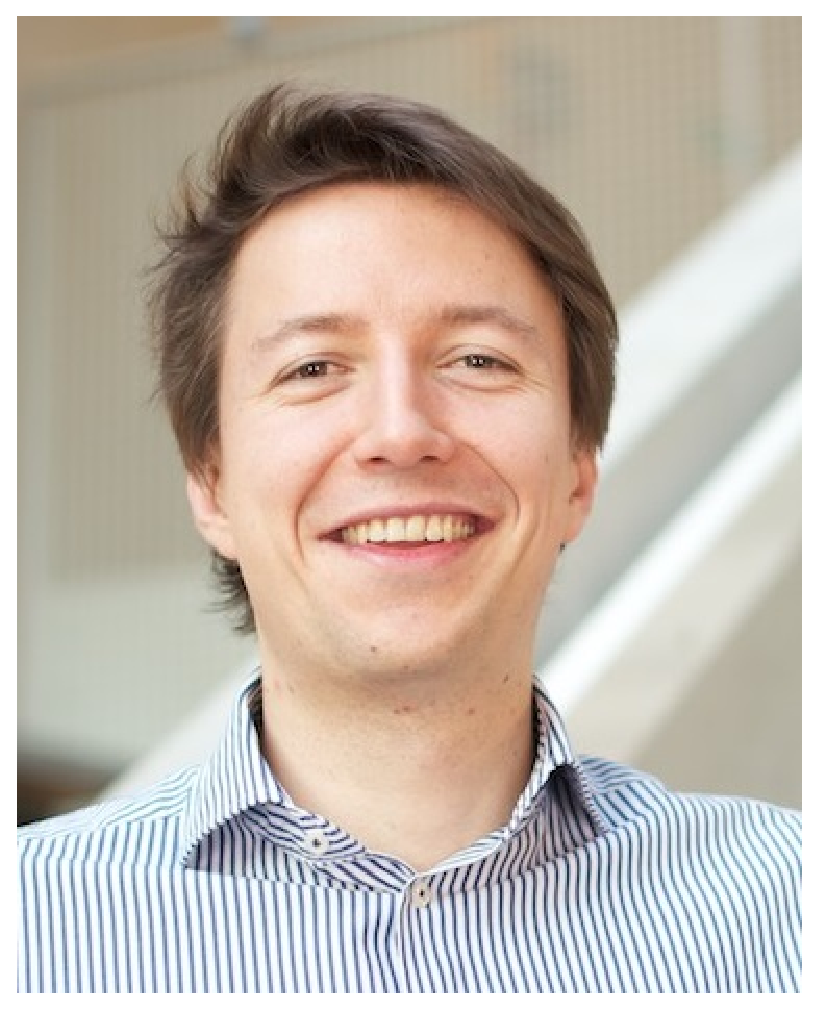
\includegraphics[height=1in]{images/vitae/ckloss}}
\noindent {\bf Christoph Kloss} received his Diploma in Mechatronics in 2007 and his PhD in Computational Fluid Dynamics in 2011, 
both at the Johannes Kepler University in Linz. From 2011 to 2014, he has been Senior Research Associate at the Department of 
Particulate Flow Modelling at the Johannes Kepler University (JKU), where he headed a DEM and CFD-DEM modelling team together 
with Dr. Goniva. Dr. Kloss is co-founder and core developer of the ``CFDEM\textregistered project'', where he is heading the development of the open source DEM code LIGGGHTS\textregistered
Dr. Kloss and Dr. Goniva founded DCS Computing in January 2012. DCS is now a leading company in providing simulation software, 
products and services in the field of DEM and CFD-DEM simulations for a variety of industries. Dr. Kloss is currently holding the position as director of DCS Computing.

\vspace{2cm}

\parpic{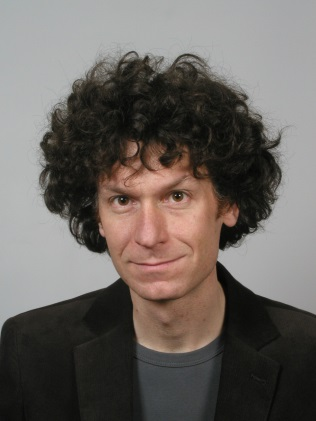
\includegraphics[height=1in]{images/vitae/spirker}}
\noindent {\bf Stefan Pirker} received his PhD in Computational Fluid Dynamics in 2001 at the Johannes Kepler University in Linz/Austria. 
In 2009 he was awarded a Christian-Doppler Laboratory on Particulate Flow Modelling, focusing on numerical modelling of particle laden flows. 
This involves development, experimental validation, application and finally open source distribution of hybrid particle laden flow models. 
After his habilitation in 2011, Stefan Pirker is currently heading the Department of Particulate Flow Modelling at the Johannes Kepler University in Linz/Austria.
